\documentclass[../main.tex]{subfiles}
\begin{document}
\part*{Results}

The Results section of the document showcases the functionality of the AWS-based image classification system. The user interface of the web application comprises a simple web page that allows users to upload any number of images for classification as shown in Figure~\ref{fig:ui} . The UI has a "Choose file" button that enables users to select the image files to be uploaded, and an "Upload" button to upload them to the AWS services.
\begin{figure}[h!]
\centering

\includegraphics[scale=0.36]{images/ui.png}
\caption{User Interface.}
\label{fig:ui}
\end{figure}

Upon clicking the "Upload" button, the web application automatically creates EC2 instances based on the number of uploaded images. A screenshot of Figure~\ref{fig:ins} displays the number of instances running based on the number of images uploaded, here . This dynamic scaling of the App-tier instances ensures that the system can handle a large number of requests efficiently.
\begin{figure}[h!]
\centering
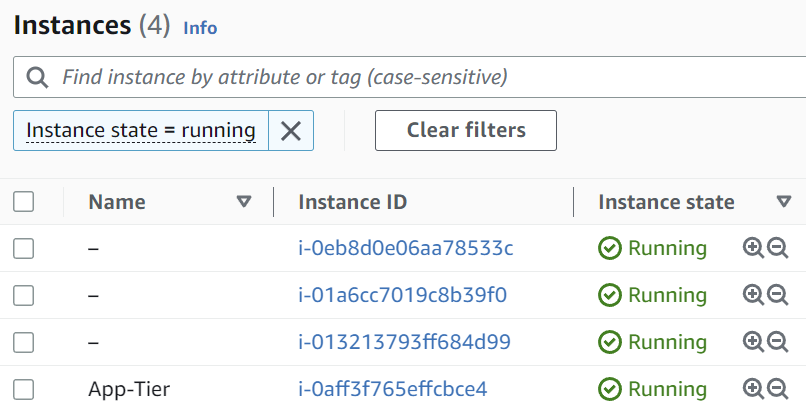
\includegraphics[scale=0.7]{images/ins.png}
\caption{4 instances are running when 3 images are uploaded.}
\label{fig:op}
\end{figure}

After the images have been processed, the system returns the classification results in the form of key-value pairs. The screenshot of Figure~\ref{fig:op} displays the results beneath the "Upload" button on the same webpage. Each image is labeled with its corresponding class and displayed in the format: \verb|test_0.JPEG, hair_spray|. This user-friendly interface enables users to quickly and easily classify multiple images with high accuracy, thanks to the use of a pre-trained ResNet model.
\begin{figure}[h!]
\centering
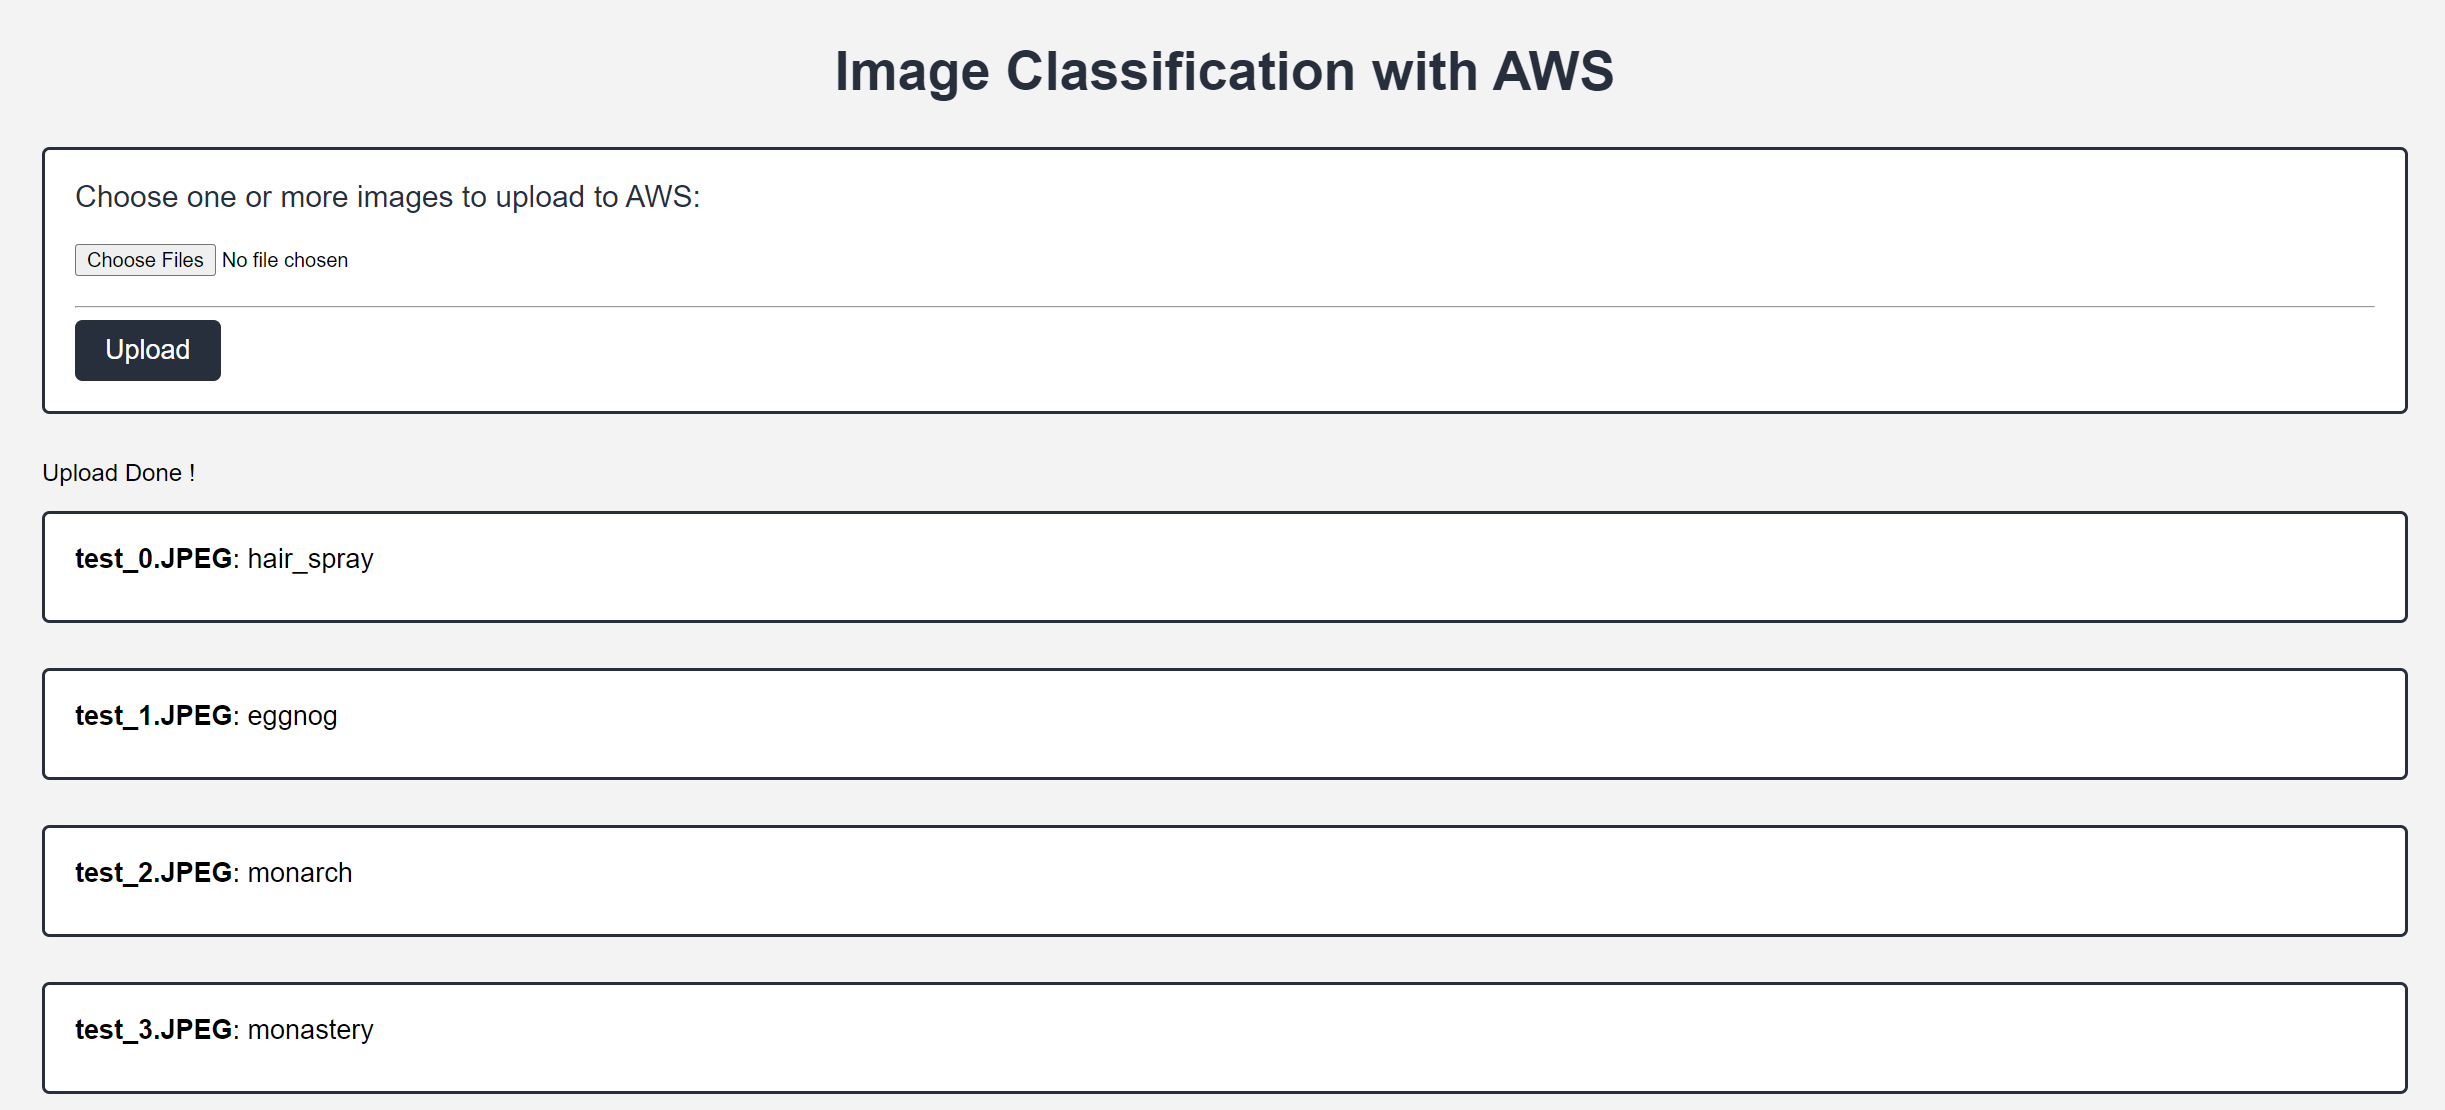
\includegraphics[scale=0.36]{images/output.png}
\caption{Sample output displayed on the UI.}
\label{fig:op}
\end{figure}

The total time taken to print the results on the webpage is calculated by measuring the time difference between two events: the first event is the time when the user clicks the upload button to initiate the image classification process, and the second event is the time it takes to display the results on the webpage. This time difference is calculated using the Python \verb|'time'| module, which provides functions to measure time in seconds. By subtracting the start time from the end time, we can determine the total time taken to print the results on the webpage.

\end{document}
\clearpage